\section{نتیجه‌ها}\label{sec:results}
این بخش نمونه‌ای از شکل، جدول و ارجاع به منبع است. شکل~\ref{fig:success} نرخ موفقیت را نشان می‌دهد
و جدول~\ref{tab:levels} سه سطح دستور را خلاصه می‌کند. کتاب \lr{\TeX} را \lr{Knuth} نوشته است~\cite{knuth1984}.

\begin{figure}[tbp]
\centering
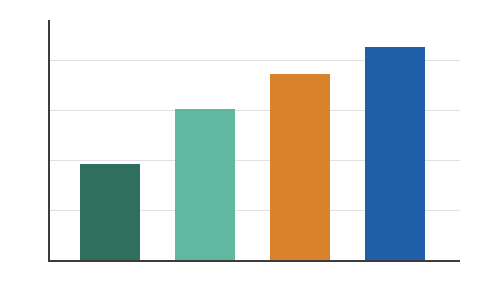
\includegraphics[width=0.6\textwidth]{figs/success-rate.png}
\caption[نرخ موفقیت چهار روش]{نرخ موفقیت چهار روش روی مجموعهٔ آزمون. هر ستون یک روش است.}
\label{fig:success}
\end{figure}

\begin{table}[tbp]
\centering
\caption[سه سطح دستور]{سه سطح دستور و معیار هر کدام.}
\label{tab:levels}
\begin{tabular}{ccc}
\toprule
سطح & نمونه & معیار\\
\midrule
اتمی & باز کردن یخچال & نرخ موفقیت\\
ترتیبی & برداشتن و گذاشتن & درستی ترتیب\\
\bottomrule
\end{tabular}
\end{table}
